\chapter{Základní problematika virtualizace síťových funkcí}
Jak již vyplývá z názvu, tak tato kapitola se zabývá základní analýzou a popisem problematiky spojené s oblastí virtuální síťových funkcí. 

Produkční vývoj v telekomunikačním průmyslu se tradičně řídil přísnými standardy kvůli stabilitě a kvalitě komunikace. Přestože tento model v minulosti fungoval, tak vedl nevyhnutelně k dlouhým produkčním cyklům, pomalému tempu vývoje a spoléhání se na proprietární či specializovaný hardware. S příchodem výrazné konkurence v komunikačních službách, od rychle postupujících organizací operujících ve velkém měřítku na veřejném internetu, podnítil poskytovatele služeb pro hledat nových způsobů, jak změnit dosavadní způsob produkčního vývoje.

Pro vyřešení toho problému bylo navrženo v publikacích \cite{NFV_paper2012} a \cite{NFV_paper2013} skupinou několika telekomunikačních provozovatelů řešení ve formě virtualizace síťových funkcí (network functions virtualization). Toto řešení má za cíl zlepšit následující aspekty provozu telekomunikačních sítí:

\begin{itemize}
\item Smíření investičních nákladů – snížení potřeby nákupu jednoúčelových hardwarových zařízení, možnost platby pouze za využité kapacity a snížení rizik přílišného předimenzování kapacit
\item Snížení provozních nákladů – snížení prostoru, napájení a požadavky na chlazení, zjednodušení správy a řízení síťových služeb
\item Urychlení Time-to-market – zkrácení doby pro nasazení nových síťových služeb, chopení se nových příležitosti na trhu, vyhovění potřebám zákazníka
\item Doručit agilitu a flexibilitu – možnost rychle škálovat (rozšiřovat nebo zmenšovat služby) dle měnících se požadavků od zákazníka. Podpora služeb, které mají být dodány pomocí softwaru na libovolném standardním serverovém hardwaru
\end{itemize}

Jak je uvedeno v \cite{NFVState} a \cite{NFVChalanges}, tak celá myšlenka je založena na tom, že dojde k separování softwarové funkcionality v síťových prvcích od proprietárního hardwaru, na kterém běží. To umožní se síťovými funkcemi zacházek jako s klasickými softwarovými aplikacemi, které mohou běžet na standardním komerčně dostupných serverech jenž organizace v současnosti používají. Tím bude zároveň umožněno flexibilní nasazování těchto síťových funkcí a jejich dynamický provisioning. Díky tomu, že jsou síťová funkce odděleny od hardwaru, tak je také možné jejich vhodnější umístění v topologii. To znamená dle požadavků na umístění mohou být nasazeny v datových centrech, síťových uzlech či přímo v uživatelově koncovém bodě. Hlavní koncept virtualizace síťových funkcí znázorňuje obrázek č. \ref{fig:vize_NFV}. 

\begin{figure}[h]
\begin{centering}
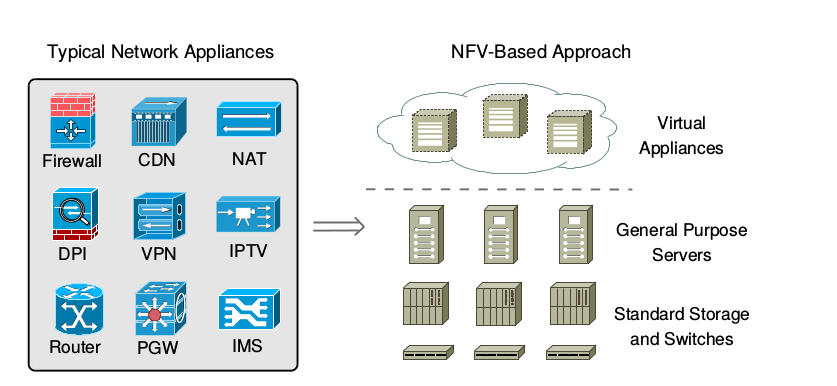
\includegraphics[scale=0.5]{images/vize_NFV}
\par\end{centering}
\caption{Koncept virtualizace síťových funkcí (NFV)\label{fig:vize_NFV}}
\end{figure}

Z zmínění stojí poznámka v \cite{NFVState}, kde je řečeno, že obecný koncept oddělení síťové funkce od hardwaru ještě nutně neznamená potřebu využití virtualizace. Protože budou síťové funkce dostupně jako software, tak mohou být nainstalovány a provozovány přímo na fyzickém stroji. Ovšem rozdíl je, že tento stroj již nebude speciální hardware, ale klasický server. Tento scénář může být do jisté míry použit při nasazovaní síťových funkcí v malém měřítku např. v uživatelských koncových bodech. Avšak pro plné využití všech výše zmíněných výhod, které jsou třeba ve velkých datových centrech, je třeba s použitím virtualizace počítat. To vše umocňuje fakt, že většina datových center v současnosti již využívá cloud computing.

Pro lepší pochopení a přehlednost celé této práce zde budou rozlišeny následující pojmy, se kterými se lze také setkat v odborné literatuře a které budou dále v této práci používány. 

\begin{itemize}
\item Síťová funkce (Network function - NF) - Toto je komponenta síťové infrastruktury, která má dobře definované funkční chování, jako například směrování, NAT, Load balancing, Intrusion detection, atd.
\item Virtuální síťové funkce (Virtual network function - VNF) - Je stejná jako NF, ale zde je funkčnost implementována pomocí softwaru a je nezávislá na hardwaru, na kterém běží.
\item Virtualizace síťových funkcí (Network Functions Virtualization - NFV) - Zde se jedná o označení celého konceptu či frameworku.
\end{itemize}

\section{NFV a Cloud Computing}

Cloud Computing a virtualizace obecně jsou hlavní technologie, které umožnily virtualizaci síťových funkcí. Z toho důvodu zde budou stručně představeny. 

Virtualizací obecně označujeme techniky, které umožňují k dostupným hardwarovým zdrojům přistupovat jiným způsobem, než jakým fyzicky existují. Je tomu díky softwaru, který tento hardware abstrahuje a vytvoří tím virtuální prostředí. Virtualizované prostředí se dá snadněji přizpůsobit potřebám uživatelů, případně skrýt pro uživatele nepodstatné detaily (jako např. rozmístění hardwarových prostředků). Tento software se nazývá hypervisor.\cite{VM_book}

Jak zmiňuje \cite{VM_architektura}, tak existují tyto dva základní typy hypervisorů:

\begin{itemize}
\item Typ 1 (Nativní) - Tento hypervisor běží přímo na fyzickém hardwaru. Tím umožňuje provozovat více operačních systému na jednom fyzickém stroji. Příkladem takového hypervisoru je VMware ESXi a XEN.
\item Typ 2 (Hostovaný) - Na rozdíl od předchozího případu tento typ hypervisoru běží v prostředí operačního systému. Příkladem je například KVM či Microsoft Hyper-V
\end{itemize}

\begin{figure}[h]
\begin{centering}
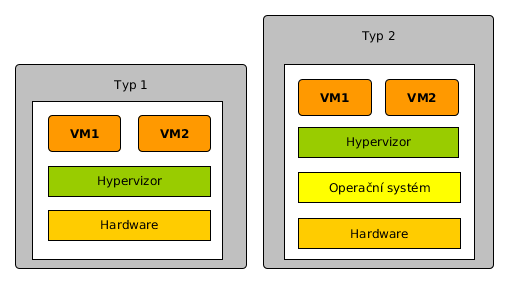
\includegraphics[scale=0.5]{images/virtualization}
\par\end{centering}
\caption{Schéma hypervisorů \label{fig:virtualization}}
\end{figure}

Obrázek \ref{fig:virtualization} zobrazuje schématický popis obou hypervisoru a jejich rozdíl. Problematika virtualizace je velice rozsáhlá a více informací o ní poskytují zdroje \cite{VM_book} a \cite{VM_architektura}.

Cloud Computing je nejpokročilejší formou virtualizace, kterou v poslední době začala provozovat většina větších organizací, jak ukazuje \cite{Cloud_adoption}. Definici cloud computingu uvádí \cite{Cloud_definice} jako 

Existuje několik modelu nasazení cloudových platforem.

\subsection{Modely nasazení}

\subsection{Distribuční modely}


\section{NFV a SDN}

\section{Architektura NFV a VNF}

Jak již bylo zmíněno, tak cílem této práce je navržení 
V předchozí sekci byla popsána myšlenka a motivace související s virtualizací síťových funkcí. Pro úspěšné splnění těchto záměrů byla v \cite{NFV_architektura} navržena referenční architektura pro framework virtualizace síťových funkcí (NFV framework). !!! Jedná se pouze o funkční návrh bez náznaků konkrétní implementace. 

\begin{figure}[h]
\begin{centering}
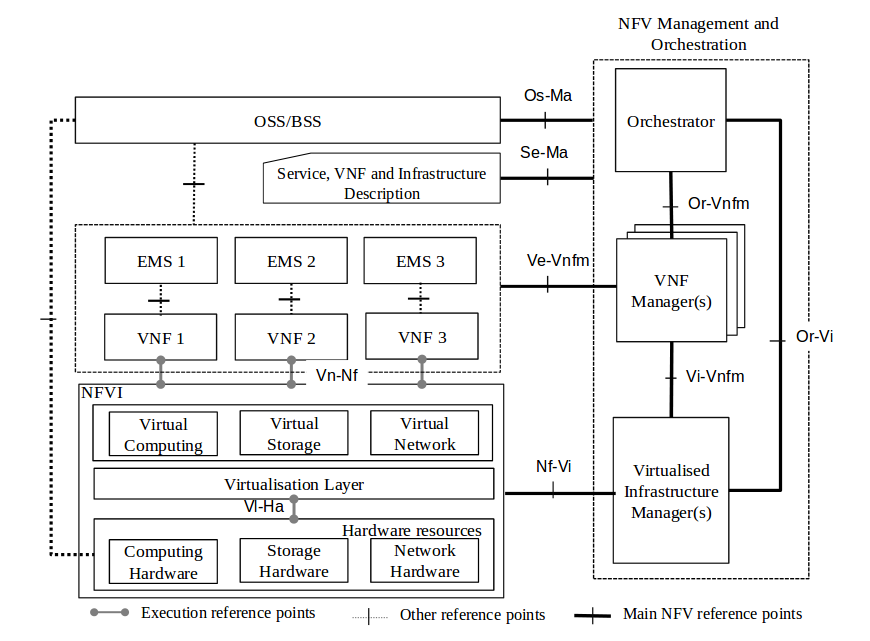
\includegraphics[scale=0.5]{images/NFV_architektura}
\par\end{centering}
\caption{NFV architektura, převzato z \cite{NFV_architektura}\label{fig:NFV_architektura}}
\end{figure}

Jak je vidět na obrázku č. \ref{fig:NFV_architektura}, tak celá architektura se dá rozdělit na tyto 3 hlavní části:

\begin{itemize}
\item Infrastruktura virtualizace síťových funkcí (NFVI) - Jsou všechny softwarové a hardwarové zdroje potřebné k vytvoření prostředí, ve které mohou být jednotlivé VNF být nasazeny. Tato infrastruktura může být velice rozsáhlá, proto je její součástí i síť poskytující konektivitu mezi vzdálenými lokacemi infrastruktury.\cite{NFV_terminology}
\item Virtualizované síťové funkce (VNFs) - Jsou softwarové implementace síťových funkcí, jako je např. NAT a routing. které mohou být nasazeny na NFV infrastruktuře.
\item Management a orchestrace NFV (NFV-MANO) - zde se jedná o řízení softwarových a hardwarových zdrojů v celé infrastruktuře NFV a životního cyklu jednotlivých virtuálních síťových funkcí. Tato část se tedy zaměřuje na řízení a správu všech úloh související v virtualizací v NFV frameworku. \cite{NFV_terminology}
\end{itemize}

Tyto funkční bloky se ještě dále dělí, proto dále v této práci budou tyto jednotlivé části popsány podrobněji a současně k nim budou uvedeny různé možnosti řešení.

\subsection{Infrastruktura NFV}

Ve zdroji \cite{NFV_infrastructure}, který detailně popisuje infrastrukturu pro virtualizaci síťových funkcí (NFVI), je uvedeno, že je v ní sdružení všech základních zdrojů potřebných pro běh virtuálních síťových funkcí (VNF). Z tohoto důvodu sem patří veškerý hardware. Do NFVI také patří některé softwarové komponenty, které jsou společné mnoho VNF a poskytují funkcionalitu potřebnou pro podporu nasazení, propojení či managementu VNF. Celou infrastrukturu může tvořit jeden či více strojů, které mají tyto potřebné funkce. Tyto stroje také mohou být umístěny v různých spolu spojených lokacích. 

Pro zjednodušení lze celou NFV infrastrukturu rozdělit do 3 následujících domén:

\begin{itemize}
\item Compute Domain - Do této domény patří veškeré hardwarové zdroje jako jsou servery, úložiště a komponenty, které tyto zdroje obsahují, např. procesory, pevné disky, síťové karty, atd. Zároveň je zde řešen návrh fyzické topologie. \cite{NFV_compute}
\item Hypervisor Domain - Toto je doména, které představuje softwarové prostředí abstrahující hardware v compute doméně a poskytuje je jako virtuální zdroje. Tyto zdroje následně mohou využívat virtuální síťové funkce. \cite{NFV_hypervisor}
\item Infrastructure Network Domain - V této doméně je řešeno veškeré propojení výše zmíněných domén. Tedy fyzické i virtuální infrastruktury.\cite{NFV_network}
\end{itemize}

Funkci obsaženou v jednotlivých doménách znázorňuje obrázek č. \ref{fig:infrastruktura}. Detailní popis těchto domén je nad rámec této práce. Více informací na tuto problematiku lze nalézt v \cite{NFV_infrastructure} a ve zdrojích uvedených u každé domény. Dá se však říci, že návrh infrastruktury pro NVF je podobný jako pro návrh infrastruktury pro cloud computing platformu. Měl by se tedy skládat z generických a komerčně vysoce dostupných serverů, na které je nasazen jeden z dostupných hypervisorů jako je např. KVM, Hyper-V či VMware. Tyto servery by následně měli být zapojeny do switche a tím by měla být zajištěna konektivita. 

\begin{figure}[h]
\begin{centering}
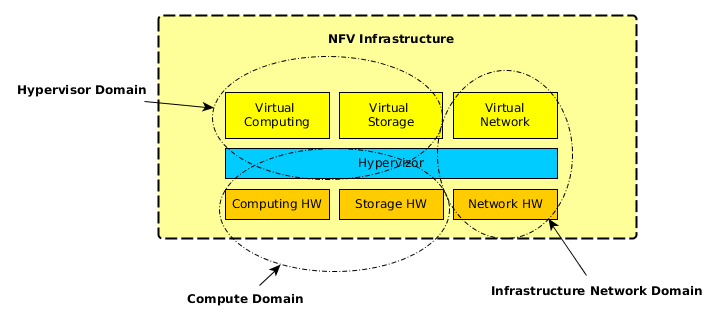
\includegraphics[scale=0.65]{images/infrastruktura}
\par\end{centering}
\caption{Schéma NFV infrastruktury\label{fig:infrastruktura}}
\end{figure}

\subsection{Virtuální síťová funkce}

Virtuální síťová funkce (VNF) je dle \cite{NFV_VNF} určitá síťová funkce, která běží na NVF infrastruktuře a je zárověň NVF frameworkem řízena a spravována. Zároveň musí mít dobře definovaný interface k ostatním síťovým funkcím, k VNF Managerovi a měla by obsahovat management interface. 

Síťové funkce jsou tedy realizovány pomocí virtuálních strojů či dnes již často používaných konteinerů. Zavisí na použité virtualizační platformě. Jedna VNF může být být obsažena v jednom virtuálním stroji nebo může být roztažena přes více virtuálních strojů. 

Na obrázku č. \ref{fig:VNF} je vidět jednoduché schéma virtuální síťové funkce. Celý životní cyklus VNF, což je vytvoření, spuštění, zastavení, smazání a škálování, řídí VNF Manager, který je součástí NVF managementu a orchestrace. Současně je možné dynamicky změnit aktuální konfiguraci pomocí Entity manageru (EM) přes management interface. EM může spravovat více VNF nebo právě jednu. Vnitřní struktura celé instance může být tvořena více komponentami (VNFC), které spolu mohou být navzájem provázány. Toto provázání však nemusí být viditelné zvenčí.

\begin{figure}[h]
\begin{centering}
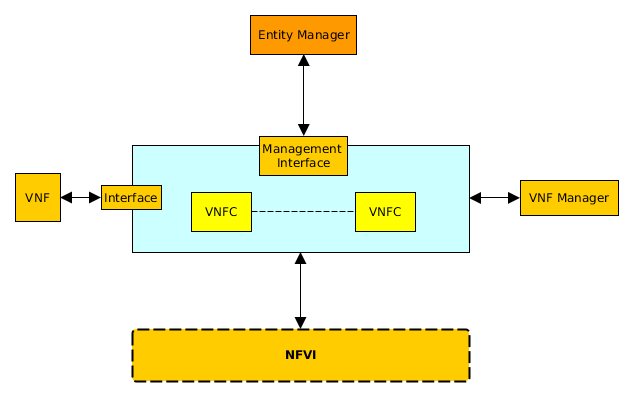
\includegraphics[scale=0.65]{images/VNF}
\par\end{centering}
\caption{Schéma virtuální síťové funkce\label{fig:VNF}}
\end{figure}



\subsection{Management a orchestrace NFV}



	\subsubsection{Orchestrator}

	\subsubsection{VNF manager}

	\subsubsection{Virtualised Infrastructure Manager}










